\section{Enabling Robots to Understand Incomplete Natural Language Instructions Using Commonsense Reasoning~\cite{DBLP:journals/corr/TesslerGZMM16}}
They introduce Language-Model-based Commonsense Reasoning (LMCR), a new method which enables a robot to listen to a natural language instruction from a human, observe the environment around it, and automatically fill in information missing from the instruction using environmental context and a new commonsense reasoning approach. Their approach first converts an instruction provided as  unconstrained natural language into a form that a robot can understand by parsing it into verb frames. 
Their approach then fills in missing information in the instruction by observing objects in its vicinity and leveraging commonsense reasoning. To learn commonsense reasoning automatically, their approach distills knowledge from large unstructured textual corpora by training a language model. Our results show the feasibility of a robot learning commonsense knowledge automatically from web-based textual corpora, and the power of learned commonsense reasoning models in enabling a robot to autonomously perform tasks based on incomplete natural language instructions. 
\begin{figure}[htbp]
    \centering
    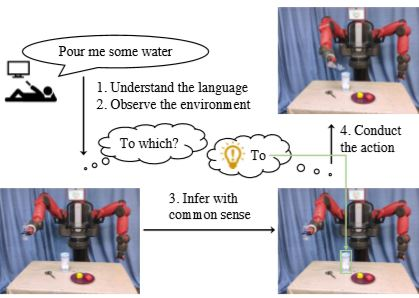
\includegraphics[width=.8\textwidth]{enable}
    \caption{A natural language controlled robot employing commonsense knowledge to interpret an instruction with missing information. }
    \label{fig:enable}
\end{figure}

A person gives an instruction “pour me some water” but the robot cannot carry out the action without knowing where to pour. After scanning the environment, the robot uses commonsense knowledge to determine the missing parameters and successfully perform the action.


